
In this section, we formulate our baseline mathematical model,
which additionally to the transmission dynamics, includes vaccination.
In order to build our  model, we follow the classical Kermack-McKendrick
approach. \Cref{Fig:SchemeModel} shows the compartmental diagram of
our mathematical model.
\begin{figure*}[tbh]
    \centering
    \includegraphics[scale = 1]{SchemeModel_0211_v3.pdf}
    \caption{%
        Compartmental diagram of COVID-19 transmission dynamics which
        including vaccination dynamics. Here, there are seven different classes:
        Susceptible $(S)$, exposed $(E)$, symptomatic infected $(I_S)$, asymptomatic
        infected $(I_A)$, recovered $(R)$, death $(D)$ and vaccinated $(V)$
        individuals. It is important to mention that $I_{S}$ represents the
        proportion of symptomatic individuals who will later report
        to some health medical center.}
    \label{Fig:SchemeModel}
\end{figure*}

Information about reinfection dynamics on COVID-19
disease is unclear to date. However, to explore some scenarios related
to this dynamic, we assume that reinfection is possible after a period
of time. On the other hand, we model the vaccination process considering
some assumptions: i) Vaccination is applied to all the alive individuals
except those in the symptomatic class. In this situation, vaccines are
applied indiscriminately over individuals on the $S$, $E$, $I_A$, and
$R$ classes; ii) the vaccine has preventive nature, that is, only
reflected in the susceptible individuals $(S)$; iii) people will only get
one vaccine during the campaign, and iv) vaccines do not necessarily have
a hundred percent of effectivity, which implies that some vaccinated people
can get the disease. We denote the effectivity rate by $\epsilon$.
Based on these assumptions our model becomes
\begin{equation}\label{model1}
    \begin{aligned}
        S'(t) &= \mu \bar{N}-\frac{\beta_S I_S +
            \beta_AI_A}{\bar{N}}S - (\mu+\lambda_V)S +
        \delta_V V+ \delta_R R
        \\
        E'(t) &= \frac{\beta_S I_S + \beta_AI_A}{\bar{N}}S+
        (1-\epsilon) \frac{\beta_S I_S+\beta_AI_A}{\bar{N}}V-(\mu+\delta_E) E
        \\
        I'_S(t) &=
        p \delta_E E-(\mu+\alpha_S) I_S
        \\
        I'_A(t) &= (1-p) \delta_E E-(\mu+\alpha_A) I_A
        \\
        R'(t)&= (1-\theta) \alpha_S I_S +
        \alpha_A I_A-(\mu+\delta_R) R
        \\
        D'(t) &= \theta \alpha_S I_S
        \\
        V'(t) &= \lambda_V S-(1-\epsilon)
        \frac{\beta_S I_S + \beta_AI_A}{\bar{N}}V - (\mu+\delta_V) V
        \\
    \end{aligned}
\end{equation}
%
where $\bar{N}(t)=S(t)+E(t)+I_S(t)+I_A(t)+R(t)+V(t)$ and
$N=\bar{N}+D$. Additionally, we include the equations
\begin{equation}
    \label{eqn:model1_counters}
    \begin{aligned}
        X'(t) &=
        \lambda_V(S + E + I_A + R)
        \\
        Y'_{I_S}(t) &=p
        \delta_E E,
    \end{aligned}
\end{equation}
where $X(t)$ and $Y_{I_S}(t)$ represent the cumulative doses at time $t$,
and the cumulative incidence at time $t$, respectively.
Parameters description of system in \Cref{model1} is provided
in \Cref{table:parametermodel}.

\begin{table*}[tbh]
    \centering
    \begin{tabular}{cl}
        \toprule
        Parameter & Description
        \\
        \midrule
        $\mu$ &  Natural death rate
        \\
        $\beta_S$ & Infection rate between susceptible and symptomatic infected
        \\
        $\beta_A$ & Infection rate between susceptible and asymptomatic infected
        \\
        $\lambda_V$ & Vaccination rate
        \\
        $\delta_{V}^{-1}$ & Immunity average time by vaccination
        \\
        $\epsilon$ &  Vaccine efficacy
        \\
        $\delta_{E}^{-1}$ & Average time of the incubation period \\
        $p$ & Proportion of symptomatic individuals  \\
        $\alpha_{S}^{-1}$ &  Average output time of symptomatic
        individuals due to death or recovery  \\
        $\theta$ & Proportion of symptomatic individuals who die due to
        the disease \\
        $\alpha_{A}^{-1}$
        & Recovery average time of asymptomatic individuals
        \\
        $\delta_{R}^{-1}$
        &  Immunity average time by disease
        \\
        \bottomrule
    \end{tabular}
    \caption{Parameters definition of system in \Cref{model1}.}
    \label{table:parametermodel}
\end{table*}

\subsection{Baseline parameters value and initial conditions}
It is now necessary to define a set of baseline parameter
values to explore some scenarios of interest. In the present work,
we consider Mexico City plus Mexico state as our study region and use
COVID-19 data to estimate some parameter values. We follow a Bayesian
approach to address this problem. We use a negative binomial
distribution as an observation model, in which the mean parameter
is given by
\begin{equation*}\label{incidence}
    \begin{aligned}
        I_{SA}(k) = Y_{I_S}(k) - Y_{I_S}(k-1)=\int_{k-1}^k p\delta_EE dt,
    \end{aligned}
\end{equation*}
where $I_{SA}(k)$ represents the incidence per day of
infected symptomatic individuals at the $k-th$ day.
The parameter estimation splits into two-stage:
before and after mitigation measures were implemented,
and we only focus on the early phase of the COVID-19 outbreak.
\Cref{Fig:fittingcurve} shows fitting curves with their respective
confidence bands for both stages. Here, we observe that our estimations
follow the growth profile of the epidemic curve. For more information about
the parameter estimation process, see \Cref{App:Parameter_Est}.
\Cref{table_icparam4} resume our parameter calibration.
%
\begin{figure*}[tbh]
    \centering
    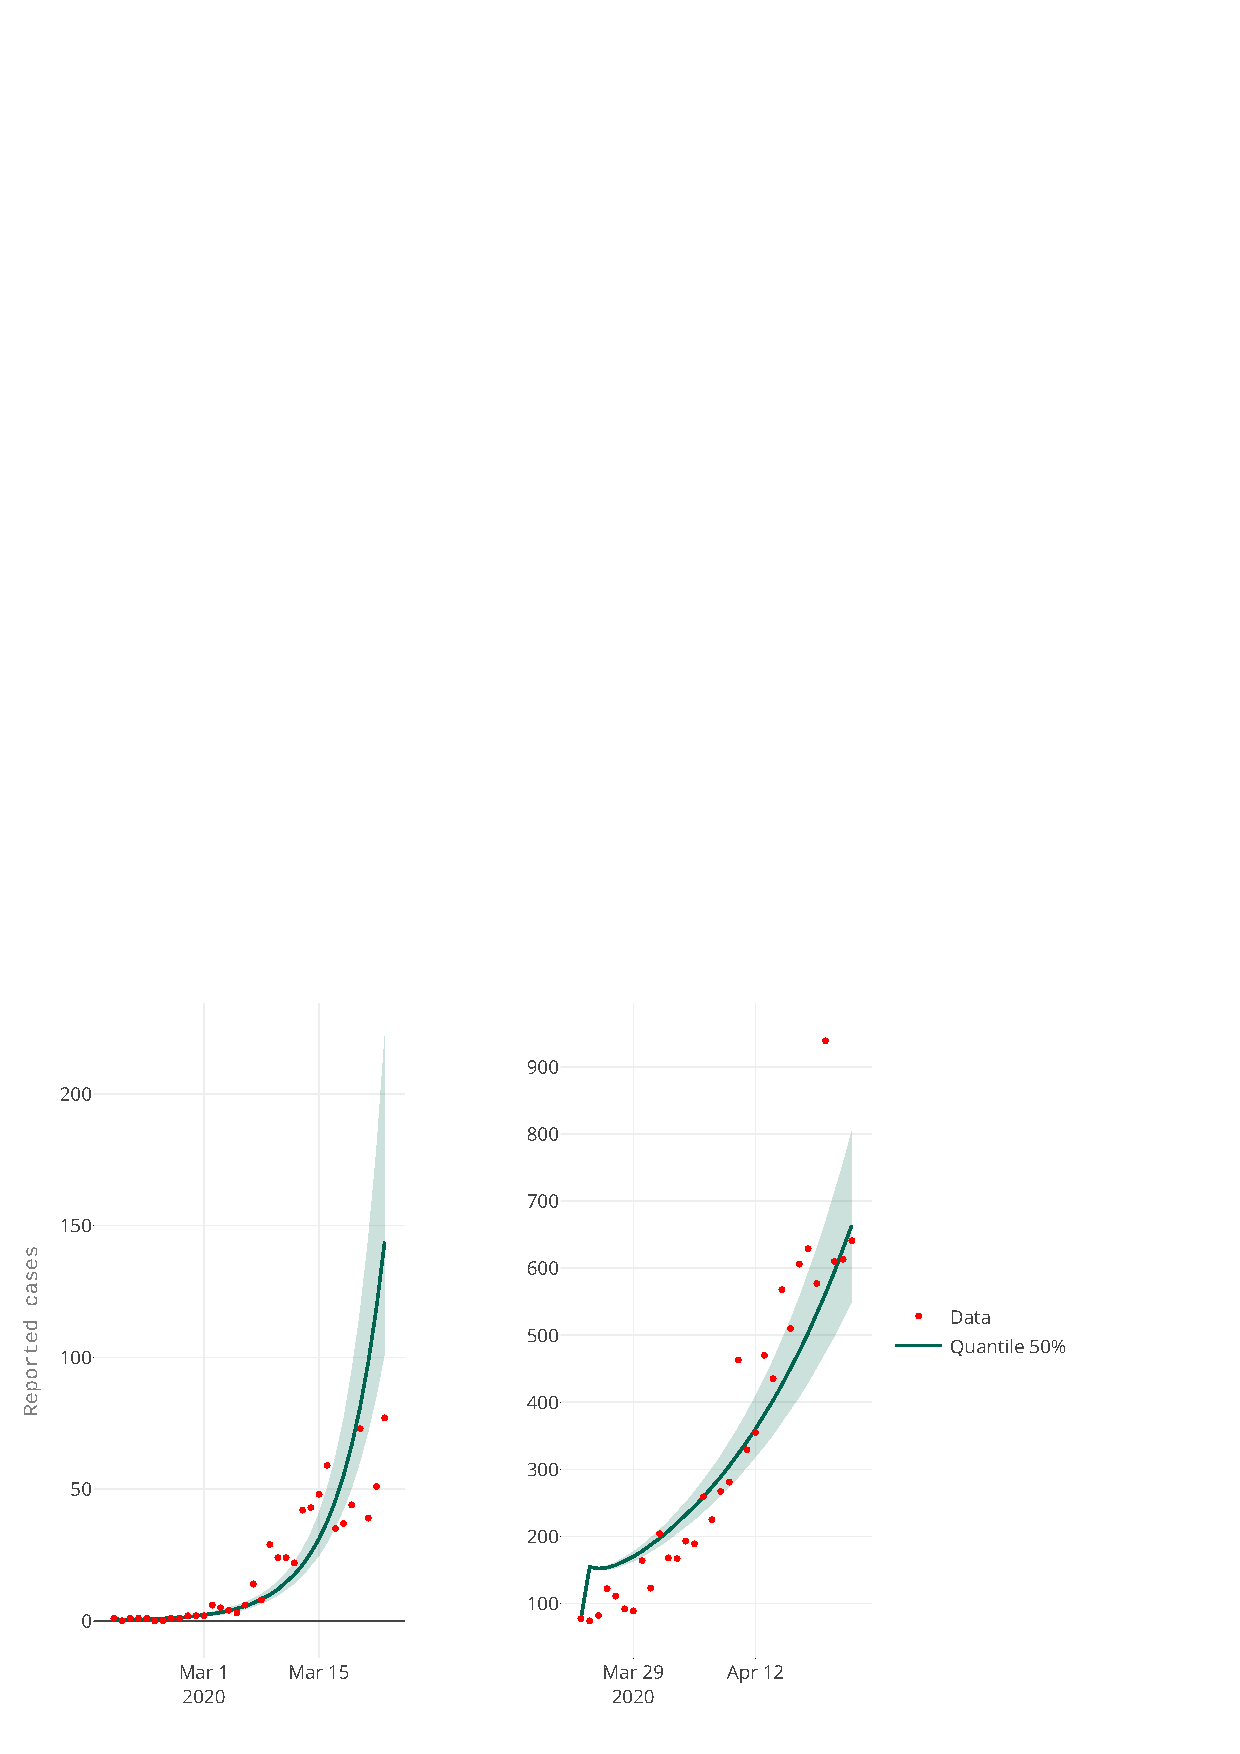
\includegraphics[scale=0.6, keepaspectratio]{FittingCurves.png}
    \caption{
        Fitting curves for the early phase of the COVID-19
        outbreak in Mexico City plus Mexico state.
        (A) Outbreak from February 19 to March 23, 2020.
        (B) Outbreak from March 23 to April 23, 2020.
        Reported data are shown in blue points, solid red line
        denote quantile 50 of all solutions
    }
    \label{Fig:fittingcurve}
\end{figure*}
%
\begin{table}[bth]
    \begin{center}
        \begin{tabular}{rl}
            \toprule
            Parameter & 95\% Confidence Interval
            \\
            \midrule
            $\beta_S$ & $[\num{0.2483712}, \num{0.48720714}]$ \\
            $\beta_A$ & $[\num{0.1851696}, \num{0.32181249}]$ \\
            $p$       & $[\num{0.061}, \num{0.2206}]$ \\
            $R_0$     & $[\num{1.702}, \num{1.887}]$\\
            \bottomrule
        \end{tabular}
        \caption{%
            Confidence interval for some parameters of system in
            \Cref{model1}, and for the basic reproductive number
            $(R_0)$.
        }\label{table_icparam4}
    \end{center}
\end{table}
%
On the other hand, since it is unclear when the vaccines will be available,
then we assume that our scenarios start on the growth stage of a second
outbreak (see \Cref{Fig:initial_conditions}) with the objective of starting
under a plausible scenario. Thus, for numerical results, initial conditions
normalized with total population
$N = \num{26446435}$, result
$S(0) = \num{0.463606046009872}$,
$E(0) = \num{0.00067033}$,
$I_S(0) = \num{0.00009283}$,
$I_A(0) = \num{0.00120986}$,
$R(0) = \num{0.532520194}$,
$D(0) = \num{0.00190074}$,
$V(0) = 0$, $X(0) = 0$, and
$Y_{I_{S}}(0) = \num{0.12258164}$.
\begin{figure*}[tbh]
    \centering
    \includegraphics[scale=0.6, keepaspectratio]{Is_dynamics.png}
    \caption{
        Dynamics of the symptomatic individuals. Black arrow indicates
        the outbreak stage in which we start our simulations.}
    \label{Fig:initial_conditions}
\end{figure*}